\documentclass[12pt]{article}
\usepackage[margin=1.27cm]{geometry}
\usepackage{setspace}
\usepackage{fontspec}
% \usepackage[T1]{fontenc}
% \usepackage[utf8]{inputenc}
\usepackage{amsmath,txfonts,amssymb,nicefrac,mathtools,pifont} %for math
\usepackage{array,tabularx,multirow,fmtcount} %for tables
\usepackage{tikz, pgfplots} %for diagram
\usepackage{multicol} %for multiple column
\usepackage{enumerate,enumitem,adjustbox} %for ordered list
\usepackage{graphicx,subcaption,wrapfig,tcolorbox} %for figure
\usepackage{xparse} %for commands & environments
\usepackage{lipsum} %miscellaneous
\usepackage{colortbl,xcolor,soul} %for default table & border

% #ANCHOR Font settings
\setmainfont{Oxygen}
\newfontfamily\banglafont[Script=Bengali]{Baloo Da 2}
\newfontfamily{\lstsansserif}{IBM Plex Mono}
\renewcommand{\normalsize}{\fontsize{11.5pt}{13pt}\selectfont}


\setlength{\arrayrulewidth}{0.35 pt}
\definecolor{border}{HTML}{A1A1AA}
\arrayrulecolor{border}


% #ANCHOR Document settings
\linespread{1.45}
\setlength\parindent{0pt}
\setlength\parskip{16pt}
\setlist[enumerate]{noitemsep}
\usetikzlibrary{shapes.geometric,decorations.pathreplacing,trees,arrows,positioning,shapes,fit,calc,decorations.markings, decorations.text}
\tikzset{every node/.append style={font=\footnotesize}}
\usepgfplotslibrary{fillbetween}
\pgfdeclarelayer{background}
\pgfsetlayers{background,main}
\pgfplotsset{compat=1.18}
\columnseprule=1pt
\everymath{\displaystyle}
% #ANCHOR Hypernation
\tolerance=1
\emergencystretch=\maxdimen
\hyphenpenalty=10000
\hbadness=10000
\newlength{\colWidth}



% #ANCHOR Colors
\definecolor{azure(colorwheel)}{rgb}{0.0, 0.5, 1.0}
\definecolor{carminepink}{rgb}{0.92, 0.3, 0.26}
\definecolor{orange}{rgb}{0.9, 0.55, 0.22}
\definecolor{violet}{rgb}{0.60, 0.45, 1}
% Syantax Highlighting Colors
\definecolor{keyword}{HTML}{D73A4A}
\definecolor{number}{HTML}{015CC5}
\definecolor{comment}{HTML}{6A737D}
\definecolor{string}{HTML}{1D825E}
\definecolor{function}{HTML}{743FD1}
\definecolor{orange}{HTML}{CF7842}
\definecolor{codeblack}{HTML}{24292F}
\definecolor{divider}{HTML}{A1A1AA}
\definecolor{border}{HTML}{D1D1D1}


% #ANCHOR Ordered & Unordered List
\setlist[itemize,1]{left=0cm, label={\textbullet}}
\setlist[itemize,2,3,4,5,6,7,8,9,10]{left=0.6cm, label={\textbullet}}
\setlist[enumerate,1]{left=0cm}
\setlist[enumerate,2,3,4,5,6,7,8,9,10]{left=0.6cm}
\setul{0.5ex}{0.125ex}



% #ANCHOR Colored Box
\let\oldul\ul
\renewcommand{\ul}[2][keyword]{\text{\setulcolor{#1}\oldul{#2}}}
\newcommand{\redbox}[1]{%
{\color{red}\fbox{\color{black}#1}}
}
\newcommand{\red}[1]{%
\textcolor{red}{#1}
}
\newcommand{\redeq}[1]{%
\text{\color{red}$#1$}
}
\newcommand{\mred}[1]{%
\textcolor{keyword}{#1}
}
\newcommand{\mredeq}[1]{%
\textcolor{keyword}{$#1$}
}
\newcommand{\blue}[1]{%
% {\color{number}#1\hspace{-0.4ex}}
\textcolor{number}{#1}
}
\newcommand{\blueeq}[1]{%
\text{\color{number}$#1$}
}
\newcommand{\cyanbox}[1]{%
{\color{teal}\fbox{\textcolor{black}{#1}}}
}
\newcommand{\cyan}[1]{%
\textcolor{teal}{#1}
}
\newcommand{\pink}[1]{%
\textcolor{magenta}{#1}
}
\newcommand{\orange}[1]{%
\textcolor{orange}{#1}
}
\newcommand{\violet}[1]{%
{\color{violet}#1}
}
\newcommand{\cyaneq}[1]{%
\text{\color{teal}$#1$}
}
\newcommand{\gray}[1]{%
\textcolor{comment}{#1}
}
\newcommand{\pinkeq}[1]{%
\text{\color{magenta}$#1$}
}
\renewcommand{\columnseprulecolor}{\color{divider}}




% #ANCHOR Tabular commands
\newcolumntype{P}[1]{>{\centering\arraybackslash}p{#1}}
\newcolumntype{M}[1]{>{\centering\arraybackslash}m{#1}}
\newcolumntype{C}{>{\centering\arraybackslash}X}
\newcommand{\rspan}[2]{\multirow{#1}{*}{#2}}
\newcommand{\thc}[1]{%
\multicolumn{1}{|c|}{\textbf{#1}}
}
\newcommand{\thcx}[1]{%
\multicolumn{1}{|C|}{\textbf{#1}}
}
\newcommand{\thl}[1]{%
\multicolumn{1}{|l|}{\textbf{#1}}
}
\newcommand{\thr}[1]{%
\multicolumn{1}{|r|}{\textbf{#1}}
}
% Adjusting arraystretch to modify vertical padding
\renewcommand{\arraystretch}{1.25}
% Adjusting tabcolsep to modify horizontal padding
\setlength{\tabcolsep}{10pt}



% #ANCHOR Math commands
\newcommand{\set}[1]{\{$#1$\}}
\newcommand{\tabs}{\ \ \ \ \ \ }
\newcommand{\tab}{\ \ \ }
\newcommand{\cmark}{\ding{51}}%
\newcommand{\xmark}{\ding{55}}%
\newcommand{\boldi}[1]{\boldsymbol{#1}}%
\newcommand{\wspace}{\ \ = \ \ }



% #ANCHOR New commands
\newcommand{\Title}[1]{%
   \begin{center}
      \textbf{\Large{#1}}
   \end{center}
}
\newcommand{\Heading}[1]{%
   \par\vspace{\dimexpr -\baselineskip + 16pt}
   {\fontsize{12pt}{13pt}\selectfont\textbf{#1}}
   \par\vspace{\dimexpr -\baselineskip + 6pt}
}
\newcommand{\BuleHeading}[1]{%
   \par\vspace{\dimexpr -\baselineskip + 16pt}
   {\fontsize{12pt}{13pt}\selectfont\textbf{\textcolor{number}{#1}}}
   \par\vspace{\dimexpr -\baselineskip + 6pt}
}
\newcommand{\CHeading}[1]{%
   \par\vspace{\dimexpr -\baselineskip + 16pt}
   \hspace{\fill}
   {\fontsize{12pt}{13pt}\selectfont\textbf{#1}}
   \hspace{\fill}
   \par\vspace{\dimexpr -\baselineskip + 6pt}
}
\newcommand{\Section}[1]{%
   \par\vspace{\dimexpr -\baselineskip + 16pt}
   \hspace{\fill}
   {\fontsize{13pt}{13pt}\selectfont\textbf{#1}}
   \hspace{\fill}
   \par\vspace{\dimexpr -\baselineskip + 6pt}
}
\newcommand{\seteqno}[1]{%
   \ \cdots \ \cdots \ \cdots \ (#1)
}
\newcommand{\eqor}{%
   \Rightarrow \ \ 
}
\newcommand{\tsub}[1]{%
\textsubscript{#1}\hspace{-0.45ex}
}
\newcommand{\tsup}[1]{%
\textsuperscript{#1}\hspace{-0.45ex}
}
\newcommand{\cbox}[2][cyan]{
\tikz\node[draw=#1,circle,inner sep=2pt,baseline=(a.base)](a){#2};
}
\newcommand{\hrline}{%
\vspace{1ex} {\color{gray}\hrule} \vspace{4ex}
}
\newcommand{\divideX}[1][divider]{{\hspace{1ex}\color{#1}{\vrule}\hspace{1ex}}}
\newcommand{\Reference}[2][Reference]{

\vspace{-0.5\baselineskip}
\begin{center}
   {\fontspec{Merriweather}\textbf{#1:} \textit{#2}} 
\end{center}
}
\newcommand{\bn}[1]{%
   {\banglafont #1}
}

\NewDocumentCommand{\Column}{O{0.49} O{1.5em} m m}{
   \setlength{\colWidth}{\linewidth-#1\linewidth-#2}
   \begin{minipage}[t]{#1\linewidth}
      \noindent
         #3
      \end{minipage}\hspace{\fill}{\color{divider}\vrule width 0.35pt}\hspace{\fill}
      \begin{minipage}[t]{\colWidth}
      \noindent
         #4
   \end{minipage}
}

% Vector commands
\renewcommand{\vec}[1]{\underline{\mathrm{#1}}}
\renewcommand{\r}{\mathrm{\textbf{r}}}
\renewcommand{\v}{\mathrm{v}}
\renewcommand{\a}{\mathrm{a}}
\let\oldkappa\kappa
\renewcommand{\kappa}{\scalebox{1.25}{$\oldkappa$}}
\newcommand{\vf}[2][t]{\vec{#2}(#1)}
\newcommand{\norm}[1]{\left\lVert\ #1\ \right\rVert}


\NewDocumentCommand{\dt}{O{t} m}{\vec{#2}^\prime(#1)}
\NewDocumentCommand{\vdt}{m}{\vec{#1}^\prime}
\NewDocumentCommand{\dtt}{O{t} m}{\vec{#2}^{\prime\prime}(#1)}
\NewDocumentCommand{\vdtt}{m}{\vec{#1}^{\prime\prime}}
\NewDocumentCommand{\vecf}{O{x} O{y} O{z}}{#1 \ \vec{i} + #2 \ \vec{j} + #3 \ \vec{k}}
\NewDocumentCommand{\vecxy}{O{x} O{y}}{#1 \ \vec{i} + #2 \ \vec{j}}
\NewDocumentCommand{\vecbf}{O{x} O{y} O{z}}{\left(#1,\ #2,\ #3\right)}
\begin{document}
\Title{Maximum \& Minimum}

\textbf{\mred{\#}} Maxima and minima of functions of two or more variables. Also find the absolute maximum and minimum in $[-6,4]$

\Heading{Solution:}

\begin{multicols}{2}
$\begin{aligned}
& f(x)=x^3+3 x^2-9 x-7 \\
& f^{\prime}(x)=3 x^2+6 x-9-0 \\
& f^{\prime \prime}(x)=6 x+6
\end{aligned}$

\columnbreak

Taking $f^{\prime}(x)=0$ to get the critical values of $f(x)$

   $\begin{aligned}
      & \Rightarrow 3 x^2+6 x-9-0 = 0 \\
      & \Rightarrow 3(x^2+2 x-3) = 0 \\
      & \Rightarrow (x+3)(x-1) = 0 \\
      & \therefore x = -3,1
   \end{aligned}$
\end{multicols}

\begin{tabular}{lll}
   At $x=-3$, & $f^{\prime \prime}(-3)=-18+6=-12$ & $12<0$ \quad so $f(x)$ is maximum at $x=-3$\\
   At $x=1$, & $f^{\prime \prime}(1)=6+6=12$ & $12>0$ \quad so $f(x)$ is minimum at $x=1$
\end{tabular}

\begin{tabular}{ll}
   Maximum value at $x=-3$ is $f(-3)$ & $= \ (-3)^3+3(-3)^2-4(-3)-7$\\
   & $= \ -27+27+27-7 \ = \ 20$\\
   Minimum value at $x=1$ is $f(1)$ & $= \ 1^3+3(1)^2-9(1)-7 \ = \ -12$
\end{tabular}


Since, $-3,1$ is in between $-6,4$. Therefore there are $4$ points $-6,-3,1,4$.

\vspace{-0.5\baselineskip}
\begin{center}
   \begin{tikzpicture}
      \draw[<->] (-3,0) -- (3,0);
      \draw (0,0.1) -- (0,-0.1) node[below] {$0$};
      \draw (-1,0.1) -- (-1,-0.1) node[below] {$-3$};
      \draw (-2,0.1) -- (-2,-0.1) node[below] {$-6$};
      \draw (1,0.1) -- (1,-0.1) node[below] {$1$};
      \draw (2,0.1) -- (2,-0.1) node[below] {$4$};
    \end{tikzpicture}
\end{center}

\vspace{-0.5\baselineskip}
Now,\\
$\begin{aligned}
& f(-6) = -216+108+54-7 = -61 \\
& f(4) = 64 + 48 -36 -7 = 69
\end{aligned}$

$\therefore$ Absolute maximum is $69$ (highest) and the absolute minimum is $-61$ (lowest)



\pagebreak
\textbf{\mred{\#}} Find the relative extrema of the function
$f(x, y)=3 x^2-2 x y+y^2-8 y$


\Heading{Solution:}
\begin{minipage}[t]{0.39\linewidth}
\noindent
   $f_x(x,y) = 6 x-2 y+0-0$\\
   $f_y(x,y) = 0-2x+2y-8$
\end{minipage}\hspace{0.5ex}{\vrule width 1pt}\hspace{0.5ex}
\begin{minipage}[t]{0.59\linewidth}
\noindent
Taking $f_x(x, y)=0$ and $f_y(x, y)=0$ to get the values of $x$ and $y$

$6 x-2 y = 0 \ \cdots (1)$ \ \ and \ \ $-2 x+2 y = 8 \ \cdots (2)$
\end{minipage}

\vspace{2ex}
Solving $(1)$ and $(2)$\\
$\begin{aligned}
6 x-2 y & =0 \\
-2 x+2 y & =8 \\
\hline 4 x & =8 \\
\therefore x & =2
\end{aligned}$

Now, \ \ $6(2)-2y \ \ \Rightarrow \ \ 12 = 2y \ \ \therefore y =6$ \tabs \tabs $\therefore$ Critical point $(2,6)$


\begin{tabular}{lccc}
   & $f_{x x}(x, y) = 6 \tabs$
   & $f_{x y}(x, y) = -2 \tabs$
   & $f_{y y}(x, y) = 2 \tabs$ \\
   At $(x, y) = (2,6)$
   & $f_{x x}(x, y) = 6 \tabs$
   & $f_{x y}(x, y) = -2 \tabs$
   & $f_{y y}(x, y) = 2 \tabs$\\
   & A & B & C
\end{tabular}

Let $D=AC-B^2 \ = \ 12-4 \ = \ 8>0$\\[-5ex]
\begin{enumerate}[label=(\alph*) \ ]
   \item if $D>0, \ \ A>0$ then $f(x, y)$ has a relative minimum.
   \item if $D>0, \ \ A<0$, the $f(x, y)$ has a relative maximum.
   \item if $D<0$, then $f(x, y)$ has a sattle point.
   \item if $D=0$, then $f(x, y)$ has no conclusion.
\end{enumerate}

But \ $A=6>0$ \ So, $f(x, y)$ has a relative minimum at $(2,6)$.


\pagebreak
\textbf{\mred{\#}} Find the relative extrema of the function
$f(x, y)=4 x y-x^4-y^4$

\Heading{Solution:}
\begin{minipage}[t]{0.39\linewidth}
\noindent
   $f_x(x,y) = 4 y-4 x^3-0$\\
   $f_y(x,y) = 4 x-0-4 y^3$
\end{minipage}\hspace{0.5ex}{\vrule width 1pt}\hspace{0.5ex}
\begin{minipage}[t]{0.59\linewidth}
\noindent
Taking $f_x(x, y)=0$ and $f_y(x, y)=0$ to get the values of $x$ and $y$

$6 x-2 y = 0 \ \cdots (1)$ \ \ and \ \ $-2 x+2 y = 8 \ \cdots (2)$
\end{minipage}

\vspace{3ex}
\begin{minipage}[t]{0.39\linewidth}
\noindent
Taking $f_x(x, y)=0$\\
$\begin{aligned}
   & 4y-4x^3 = 0\\
   & y = x^3
\end{aligned}$

\vspace{8ex}
Putting $x = -1, 0, 1$ in $y=x^3$\\
$\begin{aligned}
   & y=(-1)^3, \ \ 0^3, \ \ 1^3 \\
   \therefore \ & y=-1,0,1 \\
\end{aligned}$

\vspace{4ex}
\end{minipage}\hspace{0.5ex}{\vrule width 1pt}\hspace{0.5ex}
\begin{minipage}[t]{0.59\linewidth}
\noindent
Taking $f_y(x, y)=0$\\
$\begin{aligned}
   & 4x-4y^3 = 0\\
   & x = y^3 \ \Rightarrow \ x = (x^3)^3 \ \Rightarrow \ x^9-x = 0 \ \Rightarrow \ x(x^8-1) = 0\\
   & x=0, \quad x^8-1=0
\end{aligned}$

\vspace{4ex}
Now,\\
$\begin{aligned}
& x^8-1=0\\
\Rightarrow \ & \left(x^4+1\right)\left(x^4-1\right)=0 \\
\Rightarrow \ & \left(x^4+1\right)\left(x^2+1\right)\left(x^2-1\right)=0 \\
\Rightarrow \ & \left(x^4+1\right)\left(x^2+1\right)(x+1)(x-1)=0 \\
\Rightarrow \ & x =-1,1 \\
\end{aligned}$\\[1.5ex]
$\therefore x = 0,-1,1$
\end{minipage}

\vspace{2ex}
$\therefore$ Critical points are $(-1,-1), \ (0,0), \ (1,1)$

Now, \quad $f_{x x}=-12 x^2$ \tabs $f_{x y}=y$ \tabs $f_{y y}=-12 y^2$

\begin{multicols}{3}
$\begin{aligned}
& \text { At }(-1,-1) \\
& A=f_{x x}=-12 \\
& B=f_{x y}=4 \\
& C=f_{y y}=-12
\end{aligned}$

$\begin{aligned}
   \text{Now, } & D = AC-B^2 =144-16 \\
   & D =128>0 \\
   & A =-12<0
\end{aligned}$

$f(x, y)$ has relative max at $(-1,-1)$

\columnbreak

$\begin{aligned}
& \text { At }(0,0) \\
& A = f_{x x}=0 \\
& B = f_{x y}=4 \\
& C = f_{y y}=0
\end{aligned}$

$\begin{aligned}
\text{Now, } & D = AC-B^2 = 0 - 16\\
& D = -16
\end{aligned}$

$f(0,0)$ is a sattle point.

\columnbreak

$\begin{aligned}
   & \text { At }(1,1) \\
   & A=f_{x x}=-12 \\
   & B=f_{x y}=4 \\
   & C=f_{y y}=-12
   \end{aligned}$
   
   $\begin{aligned}
      \text{Now, } & D = AC-B^2 =144-16 \\
      & D =128>0 \\
      & A =-12<0
   \end{aligned}$
   
   $f(x, y)$ has relative max at $(1,1)$
\end{multicols}

% \mred{H.W:} $f(x,y) = x^3+y^3-63(x+y)+12xy$ is max at $(-7,-7)$ and min at $(3,3)$

\pagebreak
\textbf{\mred{\#}} Determine the dimensions of a rectangular box, open at the top, having a volume of $32 \mathrm{ft}^3$, and requiring the least amount of materials for its construction.


\vspace{2ex}
\Heading{Solution:}
\begin{multicols}{2}
   \setlength{\columnseprule}{0pt}
   \begin{center}
      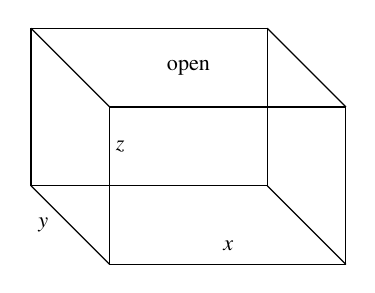
\begin{tikzpicture}
         \draw (1,0) rectangle (4,2);
         \draw (0,1) rectangle (3,3);
         \draw (1,0) -- (0,1) node[midway, left=4pt] {$y$};
         \draw (1,2) -- (0,3);
         \draw (4,0) -- (3,1);
         \draw (4,2) -- (3,3);
         \node[above=1pt] at (2.5,0) {$x$};
         \node[right=1pt] at (0.9,1.5) {$z$};
         \node at (2,2.5) {\footnotesize{open}};
       \end{tikzpicture}
   \end{center}

   \columnbreak
   Let,\\
   $x=$ length of the box in feet.\\
   $y=$ width of the box in feet.\\
   $z=$ height of the box in feet.
\end{multicols}

Therefore, Volume, $V=x y z=32$ \quad $\therefore z=\frac{32}{xy}$\\
Surface Area, $S=xy+2yz+2zx$ \quad $\Rightarrow S  =xy+2y\frac{32}{xy}+2\frac{32}{xy}x$

\vspace{-\baselineskip}
\begin{center}
   \begin{tabular}{ccc}
      $\begin{aligned}
         \therefore S_x & = y-\frac{64}{x^2}+0\\
         \therefore S_y & = x+0-\frac{64}{y^2}
      \end{aligned}$
      & \divideX &
      $\begin{aligned}
         \therefore S_{xx} & = 0-\frac{128}{x^3} \\
         \therefore S_{xy} & =1-0 \\
         \therefore S_{y y} & =0+\frac{128}{y^3}
      \end{aligned}$
   \end{tabular}
\end{center}

\vspace{-\baselineskip}
Taking $S_x=0 \ \therefore y=\frac{64}{x^2}$ \quad and \quad $S_y=0 \ \therefore  x=\frac{64}{y^2}$

\begin{center}
\begin{tabular}{rcl}
   $\begin{aligned}
     x & =\frac{64}{\left(\frac{64}{x^2}\right)^2}\\
     \Rightarrow \ \ x & =\frac{64}{64^2} \times x^4 \\
     \Rightarrow \ \ x & ^4=64 x \\
     \Rightarrow \ \ x & \left(x^3-64\right)=0 \\
     \Rightarrow \ \ x & =0,4
     \\
     \text{Since product } & xy \text{ can't be } 0.\\
     \text{Hence, } x=0 & \text{ not possible}\\
     \therefore x & =4
   \end{aligned}$
   & \divideX &
   $\begin{aligned}
& \text{Putting the value in $y$,}\\
& \therefore y =\frac{64}{4^2}=4\\
& \therefore(4,4) \text{ is the critical point}\\[4ex]
& \text{Volume } z = \frac{32}{xy} = \frac{32}{4.4} = 2
   \end{aligned}$
\end{tabular}
\end{center}

Now, at $(4,4)$\\[2ex]
\begin{tabular}{rcr}
$\begin{aligned}
   A & =S_{x x}=\frac{128}{4^3}=2\\
   B & =S_{x y}=1\\
   C & =S_{y y}=2 \quad \frac{128}{4^3}=2
\end{aligned}$
& \divideX &
$\begin{aligned}
   & D=A C-B^2=4-1=3>0 \tab \text{and} \tab A=2>0 \\
   & \text{So, } S \text{ is minimum (least amount) at} \ \ x=4 \mathrm{ft}, \ y=4 \mathrm{ft}, \text{ \ and \  }
   z=2 \mathrm{ft}\\
   & \therefore \text {Surface are, } S = xy+2yz+2zx = 4.4+2.4.2+2.2.4 = 48
\end{aligned}$
\end{tabular}

\pagebreak
\Title{Extremum Principle}
\textbf{Statement:}
Let $f(x, y)$ and $g(x, y)$ be two function of two variables $x$ and $y$ with continuous partial derivative on some open set containing the constraint curve $g(x, y)=0$ and assuming that $\vec{\nabla}g(x, y) \neq 0$ at any point on the curve. 
If $f(x,y)$ has a relative extremum at a point $(x_o, y_o)$ on the constraint curve $g(x, y)$ where the gradient vectors $\vec{\nabla} f\left(x_o, y_o\right)$ and $\vec{\nabla} g\left(x_o, y_o\right)$ this are parallel. That is, $\vec{\nabla} f=\lambda \vec{\nabla} g$, for some sealer $\lambda$. This $\lambda$ is called the \textbf{Lagrange} multiplies.

\vspace{2ex}
\textbf{\mred{7(b)}} At what points on the circle $x^2+y^2=1$ does the product $xy$ have extremum?

\vspace{2ex}
\Heading{Solution:}

\begin{multicols}{2}
   \setlength{\columnseprule}{0pt}
   $\begin{aligned}
      \text{Here, } \quad
      & f(x,y) = xy \seteqno{i}\\
      & g(x,y) = x^2+y^2=1 \seteqno{ii}\\
      \therefore
      & \vec{\nabla}f=y\vec{i} + x\vec{j} \\
      \therefore 
      & \vec{\nabla}g=2x\vec{i} + 2y\vec{j}
   \end{aligned}$

   \columnbreak

   \begin{tikzpicture}
      \draw (0,0) circle (1.5cm);
      \draw[->] (0,-2) -- (0,2);
      \draw[->] (-2,0) -- (2,0);
      \node[below left] at (0,0) {$O$};
      \node[below right] at (0,2) {$y$};
      \node[above left] at (2,0) {$x$};
   \end{tikzpicture}
\end{multicols}

\vspace{-0.5\baselineskip}
\begin{minipage}[t]{0.64\linewidth}
\noindent
   \begin{adjustbox}{valign=t}
      Set, $\vec{\nabla} g=0 \Rightarrow 2 x \vec{i}+2 y \vec{j}=0=0 \vec{i}+0 \vec{j}$
   \end{adjustbox}

   \vspace{2ex}
   From equation $(i)$ \& $(ii)$,\quad
   $2x=0 \ \therefore x=0$ \quad \quad
   $2y=0 \ \therefore y=0$

   So, $\vec{\nabla} g \neq 0$ at any points on the circle $x^2+y^2=1$\\

   $\begin{aligned}
      \text{Then }\ f(x, y) \text{ has relative extremum only when }
      & \vec{\nabla} f =\lambda \vec{\nabla}g\\
      \Rightarrow & y \vec{i}+x \vec{j} = 
      \lambda(2 x \vec{i}+2 y \vec{j})
   \end{aligned}$

Equating both side,
$y=2x\lambda \ \therefore \lambda=\frac{y}{2 x}$
\quad \text{ \ and \ } \quad
$x=2y\lambda \ \therefore \lambda=\frac{x}{2y}$
\end{minipage}\hspace{0.5ex}{\color{divider}\vrule width 0.35pt}\hspace{0.5ex}
\begin{minipage}[t]{0.341\linewidth}
\noindent
   \begin{adjustbox}{valign=t}
      \begin{tabular}{l|l}
         Now, & Then,\\
         $\begin{aligned}
         \therefore & \frac{y}{2 x}=\frac{x}{2 y} \\
         \Rightarrow & x^2=y^2 \\
         \Rightarrow & x^2-y^2=0 \\
         \Rightarrow & (x+y)(x-y)=0 \\
         \therefore \ & x= \pm y
         \end{aligned}$
         &
         $\begin{aligned}
         & x^2+y^2=1 \\
         & \Rightarrow y^2+y^2=1 \\
         & \Rightarrow 2 y^2=1 \\
         & \Rightarrow y^2=\frac{1}{2}\\
         & \therefore y= \pm \frac{1}{\sqrt{2}} \\
         & \therefore x= \pm \frac{1}{\sqrt{2}} 
         \end{aligned}$
         \end{tabular}
   \end{adjustbox}
\end{minipage}

$\therefore$ Points are
$\left(\frac{1}{\sqrt{2}},\frac{1}{\sqrt{2}}\right), \ 
\left(\frac{1}{\sqrt{2}},-\frac{1}{\sqrt{2}}\right), \ 
\left(-\frac{1}{\sqrt{2}},\frac{1}{\sqrt{2}}\right), \ 
\left(-\frac{1}{\sqrt{2}},-\frac{1}{\sqrt{2}}\right)$

\begin{tabular}{lcl}
   $\begin{aligned}
      \therefore f(x,y) &= \frac{1}{2} \text{ \tab at }
      \left(\frac{1}{\sqrt{2}},\frac{1}{\sqrt{2}}\right)\\[2ex]
      \therefore f(x,y) &= \frac{1}{2} \text{ \tab at }
      \left(-\frac{1}{\sqrt{2}},-\frac{1}{\sqrt{2}}\right)\\
   \end{aligned}$
   & \divideX &
   $\begin{aligned}
      \therefore f(x,y) &= -\frac{1}{2} \text{ \tab at }
      \left(\frac{1}{\sqrt{2}},-\frac{1}{\sqrt{2}}\right)\\[2ex]
      \therefore f(x,y) &= -\frac{1}{2} \text{ \tab at }
      \left(-\frac{1}{\sqrt{2}},\frac{1}{\sqrt{2}}\right)\\
   \end{aligned}$\\[1ex]
   \multicolumn{1}{c}{Maximum}&&
   \multicolumn{1}{c}{Minimum}
   \end{tabular}


\vspace{4ex}
\textbf{\mred{6(b)}} Find the points on the sphere $x^2+y^2+z^2=36$ that are nearest to and farthest from $(1,2,2)$.


\Heading{Solution:}
$\begin{aligned}
   \text{Let, }\quad 
   & f(x,y,z) = (x-1)^2+(y-2)^2+(z-2)^2 \seteqno{i}\\
   & g(x,y,z) = x^2+y^2+z^2-36=0 \seteqno{ii}\\
   & \therefore \vec{\nabla} f = 2(x-1) \vec{i}+2(y-2) \vec{j}+2(z-2) \vec{k} \\
   & \therefore \vec{\nabla} g = 2 x \vec{i}+2 y \vec{j}+2 z \vec{k}
\end{aligned}$

\vspace{2ex}
Set, $\vec{\nabla} g = \vec{0} \Rightarrow 2 x \vec{i}+2 y \vec{j}+2 z \vec{k}= \vec{0} = 0 \vec{i}+0 \vec{j}+0 \vec{k}$

\vspace{2ex}
\begin{tabular}{llll}
   Equating both side,&
   \ \ $2x=0$ & \ \ $2y=0$ & \ \ $2z=0$\\[-1ex]
   &$\therefore x=0$ & $\therefore y=0$ & $\therefore z=0$\\
\end{tabular}

\vspace{2ex}
So, $\vec{\nabla} g \neq 0$, at any points on the sphere.\\


\begin{tabular}{rl}
   Then $f(x,y,z)$ has relative extremum only when
   $\vec{\nabla} f$ & $=\lambda \vec{\nabla} g$\\
   $\Rightarrow 2(x-1) \vec{i}+2(y-2) \vec{j}+2(z-2) \vec{k}$ &
   $= \lambda(2x \vec{i}+2y\vec{j}+2z\vec{k})$
\end{tabular}

\vspace{2ex}
\begin{tabular}{ll|l|l}
   Equating both side,&
   \ \ $2(x-1)=2x$ & \ \ $2(y-2)=2y$ & \ \ $2(z-2)=2z$\\[0.5ex]
   &$\therefore \lambda=\frac{x-1}{x}$ & $\therefore \lambda=\frac{y-2}{y}$
   & $\therefore \lambda=\frac{z-2}{z}$\\
   & \multicolumn{3}{c}{}\\[-2ex]
   & \multicolumn{3}{c}{$\therefore \frac{x-1}{x} = \frac{y-2}{y} = \frac{z-2}{z}$}
\end{tabular}


\vspace{4ex}
\begin{tabular}{lclcl}
   $\begin{aligned}
      &\frac{x-1}{x} = \frac{y-2}{y}\\
      \Rightarrow \tab & xy-y=xy-2x \\
      \Rightarrow \tab & y=2x
   \end{aligned}$
   & \divideX &
   $\begin{aligned}
      &\frac{x-1}{x}=\frac{z-2}{z} \\
      \Rightarrow \tab & xz-z = xz-2x \\
      \Rightarrow \tab & z=2 x
   \end{aligned}$
   & \divideX &
   $\begin{aligned}
      & x^2+y^2+z^2=36 \\
      \Rightarrow \tab & x^2+4 x^2+4 x^2=36 \\
      \Rightarrow \tab & 4 x^2=36 \\
      \Rightarrow \tab & x^2=4
   \end{aligned}$\\
   \multicolumn{5}{c}{$\therefore x= \pm 2, \quad y= \pm 4, \quad z= \pm 4$}
\end{tabular}


\vspace{2ex}
$\therefore$ Points are $(2,4,4)$ and $(-2,-4,-4)$

Putting them in equation $(i)$,\\
$\begin{aligned}
   \therefore & f(2,4,4) = (2-1)^2+(4-2)^2+(4-2)^2= 1+4+4 = 9
   \text{ (nearest) \quad and}\\
   \therefore & f(-2,-4,-4) = (-2-1)^2+(-4-2)^2+(-4-2)^2 = 9+36+36 = 81
   \text{ (farthest)}
\end{aligned}$

\vspace{5ex}
\textbf{\mred{9(b)}} Find the angle between the surfaces $x^2+y^2+z^2=9$ and $z=x^2+y^2-3$ at the point $(2,-1,2)$.
\Heading{Solution:}
$\begin{aligned}
   \text{Let, }\quad 
   & f(x,y,z) = x^2+y^2+z^2=9 \seteqno{i}\\
   & g(x,y,z) = x^2+y^2-z-3=0 \seteqno{ii}\\
\end{aligned}$

\vspace{2ex}
\begin{tabular}{lcl}
   $\begin{aligned}
      & \therefore \vec{u} =  \vec{\nabla} f = 2x\vec{i}+2y\vec{j}+2z\vec{k} \\
      & \therefore \vec{v} =  \vec{\nabla} g = 2x\vec{i}+2y\vec{j}-1\vec{k}
   \end{aligned}$
   & \divideX &
   $\begin{aligned}
      & \text{At point }(2,-1,2)\\
      & \therefore \vec{u} = \vec{\nabla}f
      \ = \ 2(2)\vec{i}+2(-1)\vec{j}+2(2)\vec{k}
      \ = \ 4\vec{i}-2\vec{j}+4\vec{k} \\
      & \therefore \vec{v} = \vec{\nabla}g
      \ = \ 2(2)\vec{i}+2(-1)\vec{j}-1\vec{k}
      \quad\ \ = \ 4\vec{i}-2\vec{j}-1\vec{k}
   \end{aligned}$
\end{tabular}

\vspace{2ex}
Let $\theta$ be the angle between $\vec{u}$ and $\vec{v}$, then,\\
\begin{tabular}{lcl}
   $\begin{aligned}
      &\text{Now, }\\
      \Rightarrow \
      &\theta = \cos^{-1}\left(\frac{\vec{u}\cdot\vec{v}}{\norm{\vec{u}}\norm{\vec{v}}}\right)\\[1ex]
      \Rightarrow \
      &\theta = \cos^{-1}\left(\frac{16}{6 \sqrt{21}}\right)\\
      \therefore \
      &\theta = 54.414^{\circ}\\
   \end{aligned}$
   & \divideX &
   $\begin{aligned}
      &\text{Here, }\\
      &\norm{\vec{u}} = \sqrt{16+4+16} = 6\\
      &\norm{\vec{v}} = \sqrt{16+4+1} = \sqrt{21}\\
      &\vec{u}\cdot\vec{v} = 16+4-4 = 16
   \end{aligned}$
\end{tabular}
\end{document}